\documentclass[11pt,a4paper]{article}

% ---------------- Packages ----------------
\usepackage[margin=0.75in]{geometry}
\usepackage{times}
\usepackage{setspace}
\usepackage{enumitem}
\usepackage{graphicx}
\usepackage{booktabs}
\usepackage{array}
\usepackage{hyperref}

% ---------------- Formatting ----------------
\setlength{\parindent}{0pt}
\setlength{\parskip}{4pt}
\setlist[itemize]{noitemsep, topsep=2pt, leftmargin=18pt}
\setlist[enumerate]{noitemsep, topsep=2pt, leftmargin=20pt}

\hypersetup{
    colorlinks=true,
    linkcolor=black,
    urlcolor=blue,
    citecolor=black
}

\begin{document}

% ==================================================
%                    HEADER
% ==================================================

\begin{center}
    {\Large \textbf{23 CSE 356 SOCIAL NETWORK ANALYSIS}}\\[3pt]
    {\large \textbf{Project -- Research Proposal}}\\[8pt]

    \rule{\textwidth}{0.5pt}
\end{center}

\begin{tabular}{@{}p{0.25\textwidth}p{0.70\textwidth}@{}}
\textbf{Project Title:} & Chess Openings As Contagion \\[3pt]
\textbf{Student Name(s):} & Hridya Jain \\[3pt]
\textbf{Roll Number(s):} & [Roll Number] \\[3pt]
\end{tabular}

\vspace{5pt}
\rule{\textwidth}{0.5pt}

% ==================================================
\section*{1. Problem Statement and Motivation}

Social contagion research asks a simple question: when a person adopts a new
behaviour, how much of that is due to the people around them? The question is
hard to answer empirically because in almost every real dataset two things are
unobservable. First, \textbf{exposure} -- we rarely know whether a user actually
saw the post we assume influenced them. Second, \textbf{adoption} -- the moment a
person internally takes up a behaviour usually has no timestamp.

Online chess removes both obstacles. When an opponent plays an opening against
you, exposure is not inferred, it is forced: you had to sit at the board and
answer it. And when you subsequently play that opening yourself for the first
time, adoption is recorded exactly, to the second, in the game record. A large
public archive of online games is therefore a rare natural laboratory in which
the full exposure history and the full adoption history of millions of
individuals are both directly observable.

A network-based approach is not optional here but constitutive of the problem.
Exposure is defined by the edge structure -- who has played whom -- and the
central hypothesis concerns how many \textit{structurally distinct} neighbours an
adopter was exposed to, which is a property of the local network neighbourhood
rather than of any individual. The unit of analysis is the ego-network, not the
player.

% ==================================================
\section*{2. Research Gap}

Existing network-science work on chess treats the \textit{openings} as the
network. De Marzo and Servedio [4] construct a bipartite player--opening
structure and apply complexity algorithms to rank opening difficulty and player
skill; related work measures similarity between openings from co-play
statistics. In all of this the players are aggregated away, and the object of
study is the opening space.

Conversely, the social contagion literature has established that behaviour
spread often requires social reinforcement -- Centola's experimental result that
adoption depends on multiple independent sources of exposure [1], and Ugander et
al.'s finding that the \textit{structural diversity} of an adopter's exposed
neighbourhood predicts adoption better than the raw number of exposures [2].
These studies rely on platforms where exposure is estimated rather than
observed, and where the counterfactual is contested [3].

The gap is the intersection: no published work treats chess opening choice as a
social contagion process over the player-to-player interaction network, despite
chess offering the cleanest observable exposure signal available in any
large-scale behavioural dataset. This project addresses that gap.

% ==================================================
\section*{3. Objectives}

\begin{enumerate}
    \item To construct a temporal player-interaction network from a public
    online chess archive, and derive from it a complete, timestamped
    exposure-and-adoption record for a set of chess openings.

    \item To test whether opening adoption follows simple contagion (a single
    exposure suffices) or complex contagion (adoption probability rises with the
    number of structurally distinct exposing neighbours), by estimating adoption
    probability as a function of exposure count and exposure diversity.

    \item To separate social influence from homophily and external trends using
    a timestamp-shuffled null model and a matched-control design on player
    rating and activity.

    \item To characterise the network position of early adopters -- whether
    openings enter the population through high-centrality hubs or through
    peripheral players -- and to produce an animated visualisation of a single
    opening diffusing across the player network over time.
\end{enumerate}

% ==================================================
\section*{4. Proposed Methodology}

\begin{itemize}
    \item \textbf{Network Representation:}
    A temporal, undirected player-interaction graph $G = (V, E, T)$. Nodes $V$
    are individual players. An edge $(u, v, t)$ exists whenever $u$ and $v$
    played a game at time $t$; the same pair may be connected by many timestamped
    edges. Node attributes include rating, rating volatility and games per week
    (activity). Edge attributes include the opening played -- classified by ECO
    code and by the first $k$ plies -- the colour each player held, and the
    result. From this graph two event streams are derived: an
    \textbf{exposure event} $(A \rightarrow B, X, c, t)$, meaning $A$ played
    opening $X$ from colour $c$ against $B$ at time $t$; and an
    \textbf{adoption event} $(B, X, c, t')$, the first occasion on which $B$
    themselves plays $X$ from colour $c$, at $t' > t$.

    \item \textbf{Dataset:}
    The Lichess open game database, which publishes complete monthly archives of
    games in PGN format under a permissive licence, with persistent player
    identifiers, exact timestamps, ratings and full move lists. To keep the
    project tractable for a single investigator, the scope is restricted to one
    month of standard time-control games within a single rating band (proposed:
    1800--2200), covering the most frequent openings by ECO code. This yields a
    network on the order of $10^5$ players and $10^6$ games -- large enough for
    statistical power, small enough for a laptop.

    \item \textbf{SNA Techniques:}
    Temporal network construction and ego-network extraction for the exposure
    neighbourhoods; structural diversity measurement following Ugander et
    al.~[2], namely the number of connected components in the subgraph induced
    on a player's exposing neighbours rather than merely the count of those
    neighbours; centrality analysis (degree, betweenness, $k$-core) to test
    whether early adopters occupy distinctive structural positions; community
    detection (Louvain / Leiden) to determine whether openings diffuse
    predominantly within communities and cross between them via brokers
    occupying structural holes; null-model construction by timestamp shuffling
    and degree-preserving edge rewiring; and diffusion visualisation over the
    temporal network.

    \item \textbf{Proposed Contribution:}
    (i) A reusable pipeline that converts a raw public chess archive into an
    exposure--adoption event log over a temporal social network -- an artefact
    the contagion literature currently lacks. (ii) The first empirical test, to
    our knowledge, of simple versus complex contagion on a system in which
    exposure is directly observed rather than inferred. (iii) An identification
    strategy adapted to this setting, combining a shuffled-time null with
    rating-and-activity-matched controls, which addresses the homophily critique
    of observational contagion studies [3]. (iv) An animated diffusion
    visualisation of opening spread across the player network.

    \item \textbf{Evaluation:}
    The core measurement is the \textbf{adoption-probability curve}: the
    probability that a player adopts opening $X$ within a fixed window,
    conditioned on having received $k$ exposures from $d$ distinct opponents.
    Simple contagion predicts a curve that saturates after the first exposure;
    complex contagion predicts continued increase in $d$ while holding $k$
    fixed. Holding total exposure count constant while varying diversity is the
    decisive comparison. Validity is established by three tests: a
    \textbf{shuffled-time null}, in which permuting timestamps destroys causal
    ordering so that any residual effect is spurious by construction;
    \textbf{matched controls}, in which each exposed player is matched to an
    unexposed player of comparable rating, activity level and observation window,
    estimating the influence effect net of ``would have adopted anyway''; and a
    \textbf{predictive check}, in which a logistic model using exposure count,
    structural diversity and centrality features is evaluated by AUC on a
    held-out later time period against a baseline using opening popularity and
    player rating alone. Reported metrics: adoption-rate lift by diversity level
    with confidence intervals, effect size relative to the null, matched-pair
    difference, and held-out AUC.
\end{itemize}

% Methodology figure
\begin{figure}[h]
    \centering
    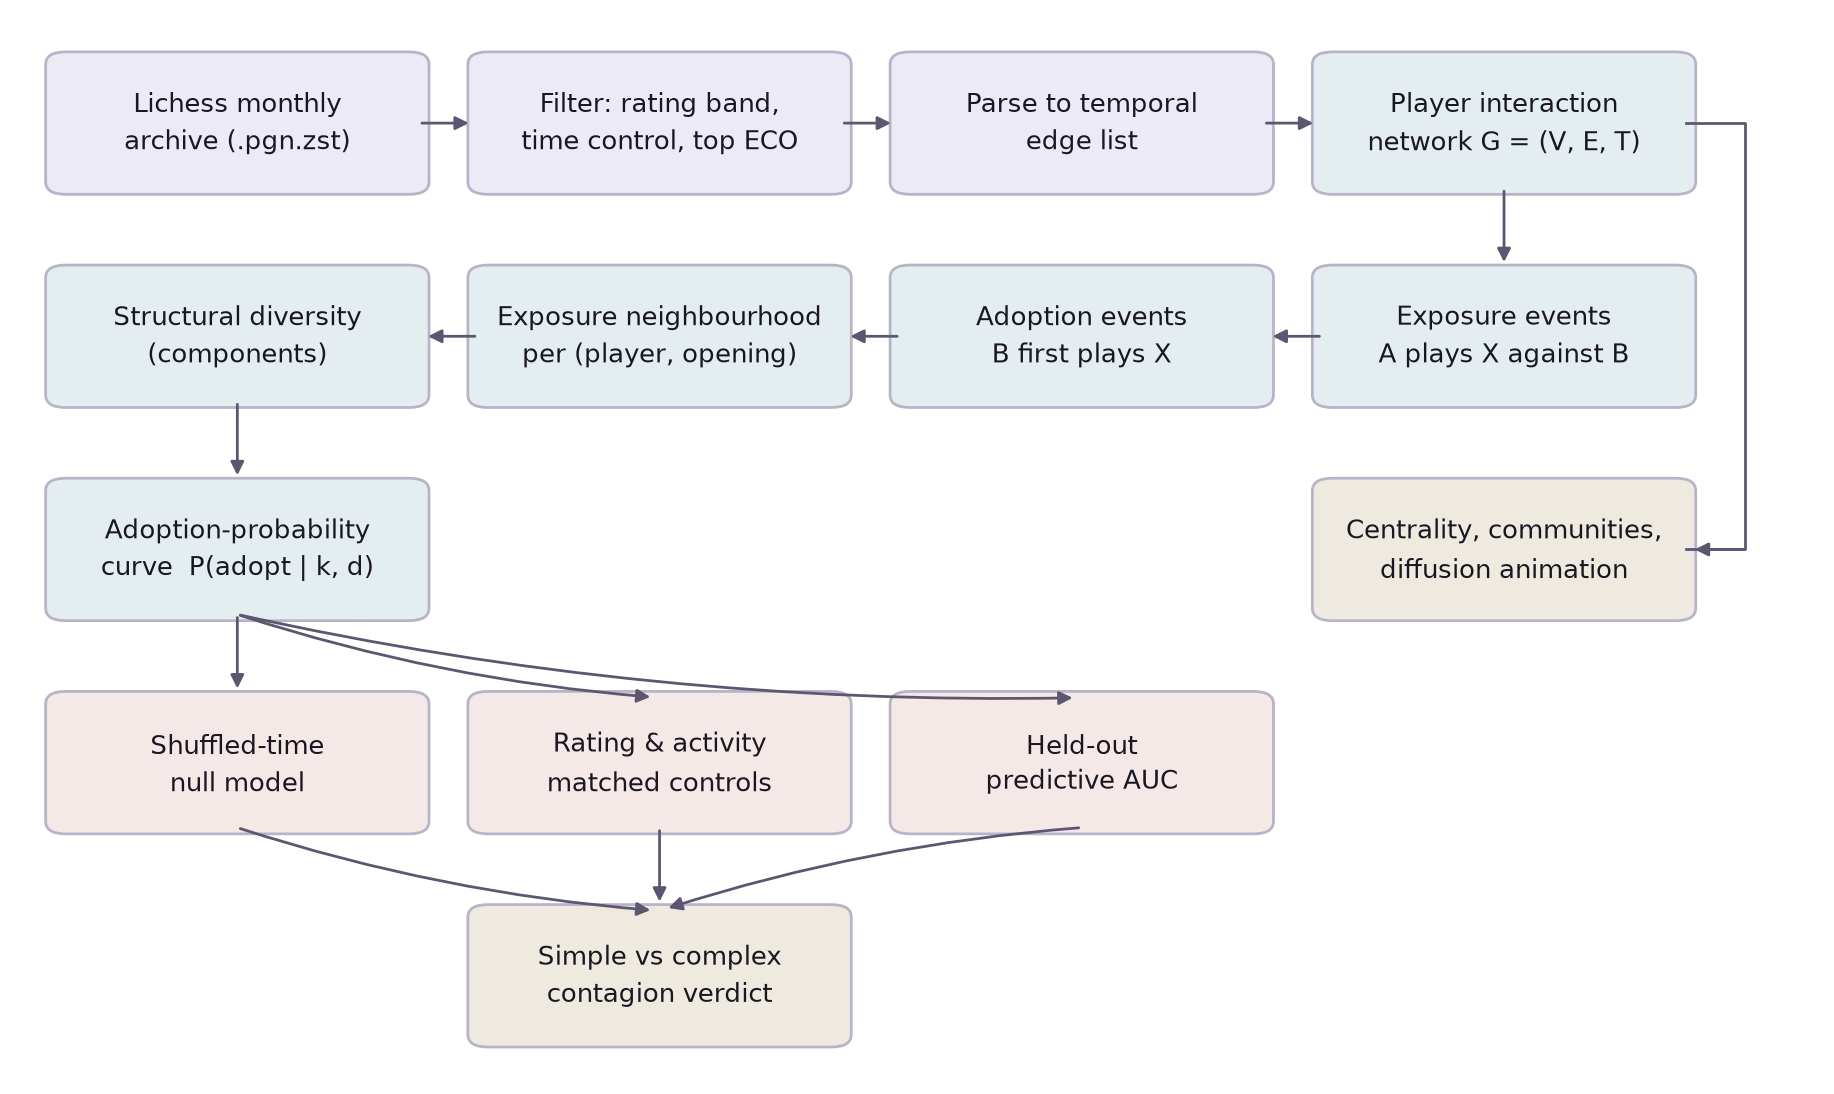
\includegraphics[width=0.95\textwidth]{figures/methodology.png}
    \caption{Overview of the proposed methodology.}
    \label{fig:methodology}
\end{figure}

% ==================================================
\section*{5. Expected Outcome}

The project is expected to produce a characterised adoption-probability curve
for chess opening uptake, and from it a defensible verdict on whether opening
choice spreads by simple or complex contagion -- a result that holds either way,
since a flat curve is as informative as a rising one. Alongside this, it will
deliver quantitative estimates of the influence effect after homophily controls,
a structural profile of early adopters relative to the wider player population,
an animated visualisation of a single opening's diffusion through the network,
and an open pipeline that converts public chess archives into contagion-ready
event logs for reuse on other openings, rating bands or platforms.

% ==================================================
\section*{6. Key References}

\begin{enumerate}[label={[\arabic*]}]
    \item D. Centola, ``The spread of behavior in an online social network
    experiment,'' \textit{Science}, vol. 329, no. 5996, pp. 1194--1197, 2010.

    \item J. Ugander, L. Backstrom, C. Marlow, and J. Kleinberg, ``Structural
    diversity in social contagion,'' \textit{Proceedings of the National Academy
    of Sciences}, vol. 109, no. 16, pp. 5962--5966, 2012.

    \item S. Aral, L. Muchnik, and A. Sundararajan, ``Distinguishing
    influence-based contagion from homophily-driven diffusion in dynamic
    networks,'' \textit{Proceedings of the National Academy of Sciences},
    vol. 106, no. 51, pp. 21544--21549, 2009.

    \item G. De Marzo and V. D. P. Servedio, ``Quantifying the complexity and
    similarity of chess openings using online chess community data,''
    \textit{Scientific Reports}, vol. 13, art. 5327, 2023.

    \item D. M. Romero, B. Meeder, and J. Kleinberg, ``Differences in the
    mechanics of information diffusion across topics: idioms, political
    hashtags, and complex contagion on Twitter,'' in \textit{Proc. 20th Int.
    Conf. World Wide Web (WWW '11)}, 2011, pp. 695--704.
\end{enumerate}

\end{document}
